\chapter{Implementation}
\section{Tech Stack Justification}
\import{chapter/05_implementation/backend}{backend_arch.tex}
\section{ Interface and Features}

Our development journey began with a thorough analysis of the client’s requirements to ensure a clear understanding of the project goals and user needs. This foundational step allowed us to identify both functional and non-functional aspects critical to delivering a seamless multilingual virtual tour assistant. Following this, we carefully evaluated and selected the most suitable technologies to meet these requirements efficiently and maintainably. To visualise the user experience and interface, we created detailed wireframes and interactive prototypes using Figma, which facilitated early feedback and iterative improvements before moving into full development.

\subsection{Client Requirements}

\textbf{Note:} We need to decide whether this section will be here or elsewhere and we have not finalized the clear requirements.

\subsection{Tech Stack Selection and Justification}

With a comprehensive understanding of the client's requirements, our next step was to carefully evaluate and select a technology stack that balances scalability, maintainability, performance, and developer experience. Each layer of the frontend architecture was considered through a comparative analysis of available tools and frameworks, ensuring that the final selections aligned with the project’s long-term goals.

\begin{table}[H]
\centering
\caption{Programming Language Comparison}
\begin{tabular}{|l|p{6cm}|p{6cm}|}
\hline
\textbf{Criteria}       & \textbf{JavaScript} & \textbf{TypeScript} \\
\hline
Typing                  & Dynamic             & Static             \\
Ease of Learning        & Easy                & Moderate           \\
Tooling Support        & Excellent           & Excellent          \\
Performance            & Good                & Good               \\
Reason                 & No static typing, harder to maintain large apps & Static typing improves code quality and maintainability \\
\hline
\end{tabular}
\label{tab:programming-language-comparison}
\end{table}

\textbf{Selected:} TypeScript \par
\textbf{Reasoning:} TypeScript was selected due to its static typing capabilities, which enhance code reliability, readability, and maintainability, especially for large-scale applications. Unlike JavaScript, TypeScript helps catch errors at compile time, making development more robust and reducing runtime bugs. It also offers better IDE support, including autocompletion and refactoring, improving developer productivity.

\vspace{2em}

\begin{table}[H]
\centering
\caption{Frontend Framework/Library Comparison}
\begin{tabular}{|l|p{4cm}|p{4cm}|p{4cm}|}
\hline
\textbf{Criteria}       & \textbf{React}                & \textbf{Angular}               & \textbf{Vue.js}               \\
\hline
Architecture            & Component-based               & Full framework                & Progressive framework         \\
Ecosystem Size          & Very Large                   & Large                        & Medium                       \\
Learning Curve          & Moderate                     & Steep                        & Easy                         \\
Performance             & Excellent                    & Excellent                    & Excellent                    \\
Flexibility             & High                         & Low                          & Moderate                     \\
Reason                  & Balance of flexibility and rich ecosystem & Steeper learning curve, more opinionated & Smaller ecosystem, less corporate support \\
\hline
\end{tabular}
\label{tab:frontend-framework-comparison}
\end{table}

\textbf{Selected:} React \par
\textbf{Reasoning:} React offers a balanced trade-off between flexibility and ecosystem maturity. Its component based architecture allows for modular and reusable UI development. Compared to Angular’s steep learning curve and opinionated structure, React provides more freedom in choosing libraries and tools. While Vue.js is simpler, React has broader community support, more enterprise adoption, and better scalability for complex applications.

\vspace{2em}

\begin{table}[H]
\centering
\caption{State Management Comparison}
\begin{tabular}{|l|p{4cm}|p{4cm}|p{4cm}|}
\hline
\textbf{Criteria}       & \textbf{Redux}              & \textbf{Zustand}              & \textbf{Context API}          \\
\hline
Boilerplate             & High                        & Low                          & Low                          \\
Learning Curve          & Steep                       & Easy                         & Easy                         \\
Performance             & Excellent                   & Excellent                    & Good                         \\
Community Support       & Very Large                  & Growing                      & Built-in React               \\
Reason                  & Powerful but verbose and complex & Lightweight, less boilerplate & Not ideal for complex state \\
\hline
\end{tabular}
\label{tab:state-management-comparison}
\end{table}

\textbf{Selected:} Zustand \par
\textbf{Reasoning:} Zustand was chosen for its minimal boilerplate, simple API, and excellent performance. It enables efficient global state management without the complexity of Redux. While Redux is powerful, it requires a steep learning curve and verbose code. Zustand fits well for modern React apps where simplicity and clarity are valued. Context API is great for light use cases but doesn’t scale effectively for complex state logic, making Zustand a better fit.

\vspace{2em}

\begin{table}[H]
\centering
\caption{Styling Solutions Comparison}
\begin{tabular}{|l|p{4cm}|p{4cm}|p{4cm}|}
\hline
\textbf{Criteria}       & \textbf{CSS}               & \textbf{Tailwind CSS}        & \textbf{DaisyUI}             \\
\hline
Approach                & Traditional                & Utility-first                & Component-based              \\
Customizability         & High                       & Medium                      & Low                         \\
Learning Curve          & Easy                       & Moderate                    & Easy                        \\
Development Speed       & Moderate                   & Fast                        & Very Fast                   \\
Reason                  & Difficult to maintain large stylesheets & Rapid styling, consistent design system & Provides prebuilt components on Tailwind \\
\hline
\end{tabular}
\label{tab:styling-solutions-comparison}
\end{table}

\textbf{Selected:} Tailwind CSS + Daisy UI \par
\textbf{Reasoning:} Tailwind CSS was selected for its utility first approach, which accelerates development and enforces consistent styling across components. DaisyUI, built on top of Tailwind, adds ready-to-use, customizable UI components that speed up design implementation. This combination reduces the need to write custom CSS while keeping the UI modern and clean. Traditional CSS is harder to scale and maintain, and DaisyUI complements Tailwind without compromising flexibility.

\vspace{2em}

\begin{table}[H]
\centering
\caption{Prototyping Tools Comparison}
\begin{tabular}{|l|p{4cm}|p{4cm}|p{4cm}|}
\hline
\textbf{Criteria}       & \textbf{Adobe XD}          & \textbf{Sketch}             & \textbf{Figma}               \\
\hline
Platform                & Desktop/Web                & macOS Desktop               & Web-based                   \\
Collaboration           & Limited                   & Limited                    & Excellent                   \\
Ease of Use             & Easy                      & Moderate                   & Easy                        \\
Prototyping Features    & Good                      & Good                       & Excellent                   \\
Reason                  & Less collaborative than Figma & macOS only, less accessible & Cloud-based, real-time collaboration \\
\hline
\end{tabular}
\label{tab:prototyping-tools-comparison}
\end{table}

\textbf{Selected:} Figma \par
\textbf{Reasoning:} Figma was chosen for its cloud-based, real-time collaboration capabilities, making it ideal for distributed teams. Unlike Adobe XD and Sketch, Figma runs entirely in the browser, requires no installation, and works across operating systems. It supports efficient design handoff with developers and includes powerful prototyping tools. Its accessibility, ease of use, and collaborative features make it the most suitable option for modern UI/UX workflows.

\vspace{2em}

\subsection{Design and Prototyping}

Design and prototyping served as a crucial bridge between client expectations and the final product. Utilizing Figma, we developed interactive wireframes and clickable prototypes to facilitate early validation, clear communication and encouraged collaborative feedback. This iterative design process helped us align the UI/UX with the multilingual and accessibility requirements of our target audience, significantly reducing rework during development.

\textbf{Note:} Will be adding more information based on figures that we are planning to add.

\subsection{Implementation}

After finalizing the Figma prototype, the implementation phase commenced and was structured into iterative sprints. Each iteration focused on delivering incremental features, incorporating design feedback, and enhancing both performance and usability. The following sections provide a breakdown of the three main development iterations undertaken.

\subsubsection{Iteration 1:}
The first iteration focused on standing up a clickable skeleton aligned to the Figma user flows. The goal was to deliver a coherent theme, working navigation, language-scoped routing, page shells for all core areas.

\begin{enumerate}
    \item \textbf{Project Setup and Theme Baseline} \\
    Initialised the project with \texttt{Next.js (App Router)}, \texttt{React}, and \texttt{TypeScript} via \texttt{npm}. Established formatting and linting rules to reduce churn. Added \texttt{Tailwind CSS} and defined a global theme (colours, spacing, type scale) applied through \texttt{globals.css}.

    \item \textbf{Routing and Internationalisation} \\
    Introduced a language-scoped route segment \verb|app/[lang]/...|. Persisted the user’s language in \texttt{localStorage} so choices survive refreshes and deep links; URLs remain shareable in the chosen language.

    \item \textbf{Application Structure} \\
    Used App Router with feature folders to separate pages and reusable components.
    \begin{itemize}
        \item \textit{Pages:} \verb|[lang]/cultural-tips|, \verb|essentials|, \verb|language|, \verb|map|, \verb|recommendations|, plus \verb|layout.tsx| and \verb|page.tsx|.
        \item \textit{Components:} \texttt{NavigationBar}, \texttt{LanguageList}, \texttt{ActionButton}, \texttt{MapComponent}, \texttt{SearchBar}, \texttt{InfoAccordion}.
        \item \textit{Support:} \texttt{mockdata/}, \texttt{public/}, \texttt{types/}, \texttt{globals.css}.
    \end{itemize}

    \item \textbf{Reusable Components (v1)} \\
    Prioritised primitives used across pages:
    \begin{itemize}
        \item \textbf{NavigationBar} — top-level navigation mounted in \verb|app/layout.tsx|.
        \item \textbf{LanguageList} — renders supported languages; writes selection to \texttt{localStorage}.
        \item \textbf{ActionButton} — shared CTA styling (``Start'', ``Change language'').
        \item \textbf{MapComponent} — visual placeholder for the map view.
        \item \textbf{SearchBar / InfoAccordion} — early building blocks for dense content.
    \end{itemize}

    \item \textbf{Page Shells Delivered} \\
    Implemented page frames with one believable mock-driven page:
    \begin{itemize}
        \item \textbf{Language selector / Change language} — same component; CTA label differs; language persisted and reflected in \verb|[lang]|.
        \item \textbf{Cultural Tips} — basic prototype rendering tips from \texttt{mockdata/}; no geo logic or filtering yet.
        \item \textbf{Map} — page shell with \texttt{MapComponent} stub and placeholder panels.
        \item \textbf{Recommendations} — placeholder cards seeded from \texttt{mockdata/}.
        \item \textbf{Essentials} — placeholder sections 
    \end{itemize}

    \item \textbf{Styling and Layout} \\
    Tailwind utilities with a global layout (\verb|app/layout.tsx|) ensure a consistent frame; \texttt{NavigationBar} renders globally. Used Tailwind’s default breakpoints; finer responsive tweaks deferred until layouts stabilised.

    \item \textbf{State and Data} \\
    No backend integration in this iteration. Used mock data to validate layouts and interactions. Persistent state limited to language via localStorage.

    \item \textbf{Stakeholder Feedback} \\
    Positive response to being able to ``click around'' immediately. Cultural Tips showed too much text at once and felt basic; requested progressive disclosure and clearer grouping.

    \item \textbf{Outcome} \\
    Delivered a navigable app matching Figma flows with a coherent theme, navigable skeleton with the language flow functional and a Cultural Tips page Map, Recommendations, and Essentials were ready for data wiring and UX refinement in subsequent iterations.
\end{enumerate}

\subsubsection{Iteration 2:}
After completing the initial development in Iteration One, the second iteration focused on refining and enhancing the existing features based on testing and client feedback. The following key tasks were accomplished during this phase:

\begin{enumerate}
    \item \textbf{Bug Fixing from Previous Iteration} \\
    Several bugs identified in the first iteration were addressed. This included UI glitches, navigation issues, and minor functional problems. All fixes were tested thoroughly to ensure stability moving forward.
    \item \textbf{Responsive Design Improvement} \\
    The entire application was reviewed and updated to ensure responsiveness across devices. Tailwind CSS utilities were used to make all pages and components adapt smoothly to various screen sizes including mobile, tablet, and desktop.
    \item \textbf{Reusable Search Bar Component} \\
    The search bar that was initially built for the language selection page was converted into a reusable, generic component. This allowed it to be used on the map page and potentially in other parts of the application, promoting code reuse and consistency.
    \item \textbf{Map Pins Integration} \\
    Pins were added to the map to represent important locations. This increased the interactivity of the map and provided users with visual cues linked to actual data and categories.
    \item \textbf{Dynamic Side Panels for Essentials and Recommendations} \\
    The static Essentials and Recommendations sections were redesigned as side panels. These panels now fetch real data from the backend API and display it with improved visual styling. Categories were introduced to organize the content better and make the user experience more intuitive.
    \item \textbf{Refining Cultural Tips}
    \begin{itemize}
        \item \textbf{Styling:} Several design mock-ups were presented to the client, and the final design was selected based on their feedback. The chosen layout was implemented with improved styling for better visual appeal.
        \item \textbf{Content Restructuring:} The earlier content was long and descriptive. It was revised and split into clear, digestible sections based on client input. The final sections include:
        \begin{itemize}
            \item Etiquette
            \item Must-know Phrases
            \item Payment Methods
            \item Transportation
            \item Emergency Numbers
        \end{itemize}
    \end{itemize}
\end{enumerate}

\subsubsection{Iteration 3:}

\begin{figure}[h]
    \centering
    \fbox{
    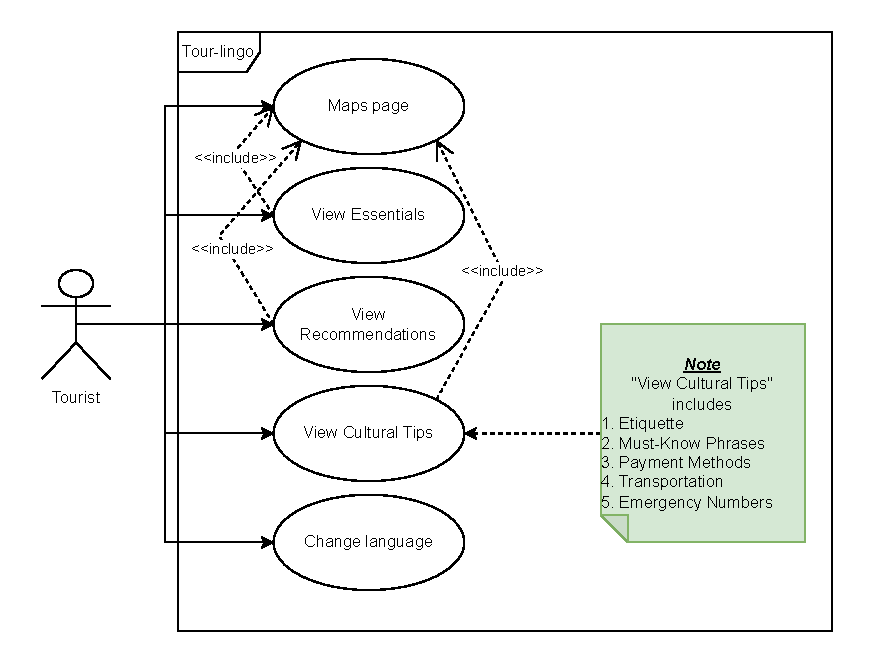
\includegraphics[width=0.5\linewidth]{chapter/05_implementation/Frontend_Usecase_Diagram.pdf}
    }
    \caption{Frontend Use Case Diagram}
    \label{fig:frontend_usecase}
\end{figure}

\section{API and Integration}
\subsection{Part of the program responsible for the map UI/UX}

\subsubsection{Fetching the data from Open Street Map }

Two major external services that we use to provide the use with navigational information are Open Street Map (OSM) and Overpass. OSM is an online and open source geographical database. The contents of the database are maintained by a community of enthusiasts and are freely accessible by everyone. However,  since the OSM does not provide a programming interface to interact with the database, our team has adopted Overpass API to solve the problem. It provides 2 types of tools that make interaction with the database possible. The first one is the interpreter that accepts the HTTP requests, that could be made via Javascript fetch api, and returns OSM database entries. Conveniently, the API supports the retrieval of OSM data in JSON format, which eases parsing through and manipulation of the fetched data. (Here we can put an example of the request form the databse) The second tool of Overpass API is the quiery lapgues, that allows for the selection of only those OSM database entries that satifsy specific characteristics. The most used feature of the query language was the selection of OSM nodes based on the tags, that explain the nature of the obejct (here we can put as an example the fetch request that retrieves only the restaurants in the area). 

When the user navigates to the map page and gives permission for his location information to be collected, an Overpass API call is made.
\begin{minted}{js} 
const fetchOverPassData = async (query: string): Promise<OverpassElement[]> => {
  const res = await fetch('https://overpass-api.de/api/interpreter', {
    method: 'POST',
    body: query,
  });
  const data = await res.json();
  return data.elements as OverpassElement[];
};
\end{minted}
!!! This specific part is work in progress, so this part could potentially be changed quite drammatically!!!

The query variable contains the Overpass query language string. It is composed with the following steps. Firstly, the list of objects containing the desired nodes is reassembles into a single string. 
\begin{minted}{js} 
 [
  { section: 'Hotel', query: 'node["tourism"="hotel"]' },
  { section: 'Restaurant', query: 'node["amenity"="restaurant"]' },
];
\end{minted}
The query specifies which exact data that is going to be retrieved. Node is one of 3 basic OSM data types (alongside ways and relations), and it represents the most basic representation of a geolocational object in the OSM database. Each data type in OSM has the following keys: "type", "id" (the serial number of the data entry), "lat" (latitude of the object) and "lon" (longitude of the object). Optionally, the objects may contain "tags" key, but becuase of the way we query the database, we will always have it. In the example "node["tourism"="hotel"]" translates to "return me all nodes, that have a 'tags' key (which value is an object), and in this object there must be a 'tourism' key, which value must be equal to 'hotel'". Conveniently, the query language supports the use of regular expressions, so the query "shop"~"supermarket|convenience|greengrocer" would return respectively the json containing the nodes referencing supermarkets, convenience stores and greengrocer stores.

The list of quieries is iterated over and a single request string is formed:
\begin{minted}{js} 
  const filterBlocks = sections
    .map((section) => `${section.query}(${bbox});`)
    .join('\n');
\end{minted}
bbox holds the bounding-box data: two longitude/latitude pairs that define the coordinates of the viewport’s boundaries for the map the user currently has open on screen. In other words, it captures the map area visible at that moment. When the single string is created, an actual databse query is composed: 
\begin{minted}{js} 
  const overpassQuery = `
            [out:json][timeout:25];
            (
            ${filterBlocks}
            );
            out center 10;
          `;
\end{minted}
The query could be translated into plain English in the following way: we want to retrieve a file in a JSON format, abort the request if it is not resolved withing 25 seconds, merge the requests for nodes with "tourism"="hotel" key and "amenity"="restaurant" key, provide latitude and longitude of this data entry no mater what the type of the OSM data entry is, and limit the final list of objects to 10 entries. 

Example of a JSON entry representing the Merchant Venturer's building:
\begin{minted}{JSON} 
{
  "type": "way",
  "id": 483814489,
  "center": {
    "lat": 51.4559134,
    "lon": -2.6029918
  },
  "nodes": [
    10739497700,
    ...
    10739497700
  ],
  "tags": {
    "addr:city": "Bristol",
    "addr:housenumber": "75",
    "addr:postcode": "BS8 1UB",
    "addr:street": "Woodland Road",
    "addr:suburb": "Cotham",
    "building": "university",
    "building:levels": "6",
    "name": "Merchant Venturers Building"
  }
}
\end{minted}

\subsection{Leaflet and interaction with the map}
1) Explain what leaflet is and how it works +  What is react-leaflet and why we need it
Leaflet is an open source JavaScript library, that provides a broad range of tools to integrate and customise an interactive map into your front-end project. In addition to adopting the Leaflet library itself, we also made use of React Leaflet API. As the name suggests, React Leaflet API adapts the Leaflet library functions to be used in a React app directly as props. (TBF this is the most I understood from reading around the topic. If someone wants to jump into the explanation how react leaflet works from React standpoint, feel free to do so)

2) Explain how our code works
- <MapContainer> prop creates the window with the rendered map itself.
- <TileLayer> prop is the one that actually imports the visual map tiles. Since have chosen the Open Street Map as a provider of geographical and locational data, we chose to utilise the interactive map from the service as well:
\begin{minted}{HTML}
<TileLayer
    attribution='&copy; 
        <a href="https://www.openstreetmap.org/copyright">OpenStreetMap</a> 
        contributors'
    url="https://{s}.tile.openstreetmap.org/{z}/{x}/{y}.png"
/>
\end{minted}
The advantage of this choice lies in the fact the the image of the map that is displayed on the screen is built on the geolocation data that OSM posesses. That means that when we query some data from the OSM database with the intent to then display/overlay it on the map, the mapping of the representation (pins) of the queried data is going to be extremely precise. On the other side, because OSM provides raster tiles (i.e prerendered PNG images of the map), extracting the names of the objects on the map, translating them and putting them back on the map essentially is impossible. It is possible to overlay the translations of the points of interest on the map, but that makes the map interface too cluttered and unappealing.

The overlaying of the desired data was done with the <Marker> prop. For example, the following code uses the information from the JSON file that was retireved with the Overpass API and converts it into the graphical information in the form of pins on the map:
\begin{minted}{HTML}
  {pins.map((pin) => (
    <Marker
      key={pin.id}
      position={[pin.lat, pin.lon]}
      icon={createSVGPin(pin.icon)}
      eventHandlers={{
        click: () => onPinClick?.(pin),
      }}
    >
      <Popup>
        <div className="p-2 leading-relaxed">
          <h3 className="font-bold text-lg mb-2 text-gray-800">
            {pin.title}
          </h3>
          <p className="text-xs text-gray-500 mb-1">{pin.category}</p>
          <p className="text-xs mb-2 leading-tight text-gray-700">
            {pin.description}
          </p>
          {pin.street && (
            <p className="text-xs text-gray-500 leading-tight mb-1">
              Street: {pin.street}
            </p>
          )}
          {pin.postcode && (
            <p className="text-xs text-gray-500 leading-tight">
              Postcode: {pin.postcode}
            </p>
          )}
        </div>
      </Popup>
    </Marker>
  ))}
\end{minted}
In this example the "pins" array of objects was created after parcing though the OSM JSON file and destructuring the useful information (e.g. entry name, address, coordinates etc.). This information is displayed to the user upon click on the pin, for which the markers <Popup> prop is responsible. 

\subsection{Nomitam API - how do we do geocoding and reverse geocoding (+ point of interest search)}
Forward geocoding (or simply geocoding), conceptually, is a transformation of a human readable address into a a latitude and longitude number tuple. Hence, reverse geocoding is a process of retrieval of the most appropriate address from the provided coordinates. Both services are standard means to interact with an online map, and there is a number of providers of the geocoding service. Considering our budget limitations and high reliance on OSM, we chose Nomitam API as a provider with an unlimited free plan and which includes high integration with OSM data. Despite the drawback of Nomitam (low volume of requests and no support for high traffic applications) for the purposes small scale development we considered it to be the perfect tool. 

In our application we use both forward and reverse geocoding. When the user navigates to the map page, the geolocation of the device of the user is collected, following permission from the user. The collection is handled by the \mintinline{js}{getCurrentPosition()} method of the Geolocation interface, which belongs to the Document Object Model (DOM) API. Once the coordinated are collected, an Nomitam API call for reverse geocoding is made with said coordinates:
\begin{minted}{js}
const res = await fetch(
  `https://nominatim.openstreetmap.org/reverse?format=json&lat=${lat}&lon=${lon}`
);
\end{minted}
Following the parsing of the response of we extract the name of the city and the country that the user is in. This data is then set as a global variable using Zustand library and used, for instance, for generation of a cultural tip by the LLM.

The forward geocoding is implemented in the map page's Search bar. When the user decides to enter any text into the searchbar, the following code is executed:
\begin{minted}{js}
useEffect(() => {
if (!searchByUser.current || searchText.length < 3) {
  setSearchResults([]);
  return;
}
const controller = new AbortController();
const timeout = setTimeout(() => {
  const fetchSearchResults = async () => {
    setIsfetching(true);
    try {
      const res = await fetch(
        `https://nominatim.openstreetmap.org/
        search?q=${encodeURIComponent(searchText)}&format=json`,
        {
          signal: controller.signal,
        }
      );
      const data: NominatimResult[] = await res.json();
      setSearchResults(data || []);
    } catch (err: unknown) {
      if (err instanceof DOMException && err.name === 'AbortError') return;
      console.error('Search error: ', err);
    } finally {
      setIsfetching(false);
    }
  };
  fetchSearchResults();
}, 100);
\end{minted}
This code could be translated into English as follows: when the user types something into the keyboard, try to match the typed text to the names of the existing map objects. If they exist, return JSON objects that would contain the information characterizing these objects. (To be fair, I could spend a couple of pages just describing how the searchbox works, because it's kinda brilliant, but in the context of API and integration, I am not sure how deep I should go tbh)


-----Don't forget about the boudning box filtering, or should I forget about it?-----

(https://community.codenewbie.org/ramesh0089/top-7-free-geocoding-apis-every-developer-should-know-in-2025-b74 -> nomitam limitations)

\subsection{how does the cultural tip work}
Introduction to the choice of the APIs.

When this feature of the application was in the early stages of development, we were attempting to integrate Wikitravel data as the source of information. The general idea was that when we get the geolocation information from the user, a web scraper would retrieve the information from the appropriate web page. This information would then be parsed, and the contents of each section (e.g. modes of transportation, landmarks, shops, cafes etc.) would be displayed for the user to explore. However, the section names varied drastically from city to city, making categorization of the information and its uniform presentation to the user near impossible. Moreover, the client decided that the feature would contain only the most essential information, and all of the UI should fit into one page. Hence, we decided to adopt the use of a Large Language Model (LLM) to generate the data for us.  Self-hosting an LLM requires the computations power in the form of a high performing GPU [reference] that our team did not possess. Therefore, we adopted OpenRouter API that handles API calls to a range of available LLMs. Importantly, OpenRouter provides access both to free-to-use and paid options of LLM use, which leaves the choice to the client to scale the application after the project ends or not.  

When the user navigates to the cultural tips page, the following API call is made. 
\begin{minted}{js} 
  const response = await fetch(
    'https://openrouter.ai/api/v1/chat/completions',
    {
      method: 'POST',
      headers: {
        Authorization: `Bearer ${process.env.NEXT_PUBLIC_OPENROUTER_API_KEY}`,
        'Content-Type': 'application/json',
      },
      body: JSON.stringify({
        model: 'mistralai/mistral-7b-instruct:free',
        messages: [
          { role: 'system', content: systemPrompt },
          { role: 'user', content: userPrompt },
        ],
      }),
    }
  );
\end{minted}
Importantly, OpenRouter implements OpenAI API specification for /completions and /chat/completions endpoints \cite{noauthor_openrouter_nodate}. Therefore, we can use OpenAI API terminology \cite{openAI_explanation_onHowToUseTheirApi} to shape the reply we get from the LLM of choice regardless of what the LLM was chosen. To instruct the LLM to provide us with the response that we can automatically parse through, the messages array contains an object { role: 'system', content: systemPrompt }. systemPrompt variable is a string that 1) explains what role the LLM should take 2) what format of data use program expects to receive 3) what shape the resulting JSON file should be in 4) how many values should each entry contain 5) what to do in case the information does not exist or is not retrievable. Conversely, in the { role: 'user', content: userPrompt } the userPrompt variable is a simple string "Generate JSON for \$\{city\}", where the city variable is a zustand (global) variable created when the user provides their location in the map page. 

Although we have included strict format rules in the system prompt to the LLM, the received data still had to be checked for sections containing data in an inappropriate format, as well as malformed/missing sections. After the format of the data is verified, a backend API call is made:
\begin{minted}{js} 
fetch(APIUrl, {
method: 'POST',
body: JSON.stringify(verifiedRequestBody),
headers: {
  'Content-type': 'application/json',
},
})
\end{minted}
where the APIUrl is the endpoint of our backend ("process.env.TRANSLATION\_API\_URL") and verifiedRequestBody is a variable that contains the object with has been properly formatted. When the API call is resolved, the data is once again verified using the cade code object checker as before. Finally, it is retured to the page.tsx, where it is parsed through and displayed to the user. 

\section{Deployment of the front end}
\subsection{Drafting notes}
What might I include here?
\begin{itemize}
    \item What is the purpose
    \item What did I have
    \begin{itemize}
        \item Pros and cons of each option
        \item What did I ended up seetling up with
    \end{itemize}
\end{itemize}

- Why need deployment in the first place
While containerisation and deployment of the backend service was a necessary step to ease the development process, the deployment of the front end was necessary for different reasons. Firstly, showcasing an application to testers/focus groups would be more frictionless when people won't have to queue up for the number of computers that have the front-end running with npm run dev. Any person who would like to have a glace at the application could simply follow a website link and start using the application from their device. The second point stems from the first one, namely, the location of people wishing to use the app doesn't matter since the only requirement to use the app is internet connection. And finally, our team was interested to know whether or not the application could be scaled easily, which would inadvertently imply deployment. 

- Deploying from Github directly (maybe try to rephrase to include that you wanted to deploy the application from github from the beginning, but you didn't want to change the code so that we wouldn't be restricted in the choice of providers).
The official Next.js documentation page \cite{vercelMainDeploymentMainPage} provided a number of options to deploy the front end. Initially, we attempted to deploy our project to Vercel \cite{Next.jsonVercel}. The reasoning behind this choice was that the Next.js framework itself was developed and maintained by Vercel (reference), and therefore it was assumed that Vercel would have the most seamless deployment process. However, the major obstable that we encountered at this step was a paywall. One of the major requirement for the entire web app that was stated from the beginning of the project was that we can only use paid software tools and cervices only if for the purposes of the project the free alternatives either don't fit or exit. Therefore, we tried to deploy the front end to the main alternative of Vercel - Cloudfare \cite{cloudflareMainPage}. Like Vercel, Cloudflare Pages and Workers have full support for deployment of Next.js project \cite{cloudflareWorkersMainPage} while having an unlimited free plan with restrictions that didn't significantly impact the project during and post development. Moreover, the platform provided high integration with GitHub, and after every merged pull request an automatic deployment to the server would be triggered, which was a nice addition. However, after setting up and attempting to deploy the project, we have encountered the issue of project not being properly configured for running on edge. After consulting the documentation for this specific issue \cite{APIReferenceEdgeRuntime}, as well as additional way to deploy the project to the same site \cite{Next.jsCloudflareDocs}, we have determined that deploying the application without addition configuration files and code snippets would not be possible. After reviewing the situation and weighing pros and cons of deploying to CloudFlare, we decided that trying to resolve all of the issues and limiting ourselves and the client to only one provider was not worth it. Therefore, we decided change our deployment strategy entirely, and deploy a docker container instead. (Can also waffle about other services having issues with deployment, but not sure if that is even necessary)

- Deploying a containerized application (it may be a good idea to docuemnt what steps I made word for work for other people to replicate waht I did)
Conveniently, Next.js documentation also provides general steps that are can be taken in successful containerization and deployment of the project \cite{vercelMainDeploymentMainPage}\cite{next.js/examples/with-docker}. Conveniently, the only two necessary additions to the code (that also didn't change how the code functioned), were the addition of the Dockerfile \cite{next.js/examples/with-docker/Dockerfile} and "output: "standalone"," line to the next.config.js file, neither of which changed how the application worked. To create an image of the project I used the command "docker build -t tour-de-face-docker .". To create and run a container from the image I use the GUI of Docker Dextop. From there, in terms of deployment there were several options to explore. The easiest and the cheapest one was to expose the localhost port to the web using Ngrok, which is a free software that promises to do this securely \cite{ngrokMain} \cite{ngrokMainDocs}. This approach had several advantages. Firstly, since the application was self-hosted (i.e. was run on one of the personal computers), it was completely free, discounting minimal energy bills that come from operating a laptop. Moreover, containerization allowed for a quick and painless change of a host device, should the need arise. The downside of self-hosting was the questionable security, as well as inability of scaling the applciation. However, for the purposes of demonstrating the application to the end user, it was a successful general proof-of-concept that our application could be deployed. Out of curiosity (mostly), we decided to find out whether the image/containter could be deployed to the cloud. Our initial choice of a cloud container runner was Google Cloud run, as it provided a quite generous free tier plan. However, since a containter runner service does not require any additional configurations unlike adapter services, if for some reason we or the client decides to switch the container runner provider, that would be a matter of uploading the image/container to the service. The major downside of using the cloud runners though is that there is no immediate and seamless way to create a continuous deployment pipeline (although I speculate that would be possible with additional tools such as GitHub actions). Another issue that we have noticed is that the 

The downside is that there is no obvious solution on how to make an automatic deployment upon push to main. (Maybe possible with github actions, but like don't fix what ain't broke)

-----------Can also create a table for the options and paste it here--------------------------------